% Options for packages loaded elsewhere
\PassOptionsToPackage{unicode}{hyperref}
\PassOptionsToPackage{hyphens}{url}
\PassOptionsToPackage{dvipsnames,svgnames,x11names}{xcolor}
%
\documentclass[
  letterpaper,
  DIV=11,
  numbers=noendperiod]{scrartcl}

\usepackage{amsmath,amssymb}
\usepackage{iftex}
\ifPDFTeX
  \usepackage[T1]{fontenc}
  \usepackage[utf8]{inputenc}
  \usepackage{textcomp} % provide euro and other symbols
\else % if luatex or xetex
  \usepackage{unicode-math}
  \defaultfontfeatures{Scale=MatchLowercase}
  \defaultfontfeatures[\rmfamily]{Ligatures=TeX,Scale=1}
\fi
\usepackage{lmodern}
\ifPDFTeX\else  
    % xetex/luatex font selection
\fi
% Use upquote if available, for straight quotes in verbatim environments
\IfFileExists{upquote.sty}{\usepackage{upquote}}{}
\IfFileExists{microtype.sty}{% use microtype if available
  \usepackage[]{microtype}
  \UseMicrotypeSet[protrusion]{basicmath} % disable protrusion for tt fonts
}{}
\makeatletter
\@ifundefined{KOMAClassName}{% if non-KOMA class
  \IfFileExists{parskip.sty}{%
    \usepackage{parskip}
  }{% else
    \setlength{\parindent}{0pt}
    \setlength{\parskip}{6pt plus 2pt minus 1pt}}
}{% if KOMA class
  \KOMAoptions{parskip=half}}
\makeatother
\usepackage{xcolor}
\setlength{\emergencystretch}{3em} % prevent overfull lines
\setcounter{secnumdepth}{-\maxdimen} % remove section numbering
% Make \paragraph and \subparagraph free-standing
\ifx\paragraph\undefined\else
  \let\oldparagraph\paragraph
  \renewcommand{\paragraph}[1]{\oldparagraph{#1}\mbox{}}
\fi
\ifx\subparagraph\undefined\else
  \let\oldsubparagraph\subparagraph
  \renewcommand{\subparagraph}[1]{\oldsubparagraph{#1}\mbox{}}
\fi


\providecommand{\tightlist}{%
  \setlength{\itemsep}{0pt}\setlength{\parskip}{0pt}}\usepackage{longtable,booktabs,array}
\usepackage{calc} % for calculating minipage widths
% Correct order of tables after \paragraph or \subparagraph
\usepackage{etoolbox}
\makeatletter
\patchcmd\longtable{\par}{\if@noskipsec\mbox{}\fi\par}{}{}
\makeatother
% Allow footnotes in longtable head/foot
\IfFileExists{footnotehyper.sty}{\usepackage{footnotehyper}}{\usepackage{footnote}}
\makesavenoteenv{longtable}
\usepackage{graphicx}
\makeatletter
\def\maxwidth{\ifdim\Gin@nat@width>\linewidth\linewidth\else\Gin@nat@width\fi}
\def\maxheight{\ifdim\Gin@nat@height>\textheight\textheight\else\Gin@nat@height\fi}
\makeatother
% Scale images if necessary, so that they will not overflow the page
% margins by default, and it is still possible to overwrite the defaults
% using explicit options in \includegraphics[width, height, ...]{}
\setkeys{Gin}{width=\maxwidth,height=\maxheight,keepaspectratio}
% Set default figure placement to htbp
\makeatletter
\def\fps@figure{htbp}
\makeatother

\usepackage{booktabs}
\usepackage{longtable}
\usepackage{array}
\usepackage{multirow}
\usepackage{wrapfig}
\usepackage{float}
\usepackage{colortbl}
\usepackage{pdflscape}
\usepackage{tabu}
\usepackage{threeparttable}
\usepackage{threeparttablex}
\usepackage[normalem]{ulem}
\usepackage{makecell}
\usepackage{xcolor}
\KOMAoption{captions}{tableheading}
\makeatletter
\makeatother
\makeatletter
\makeatother
\makeatletter
\@ifpackageloaded{caption}{}{\usepackage{caption}}
\AtBeginDocument{%
\ifdefined\contentsname
  \renewcommand*\contentsname{Table of contents}
\else
  \newcommand\contentsname{Table of contents}
\fi
\ifdefined\listfigurename
  \renewcommand*\listfigurename{List of Figures}
\else
  \newcommand\listfigurename{List of Figures}
\fi
\ifdefined\listtablename
  \renewcommand*\listtablename{List of Tables}
\else
  \newcommand\listtablename{List of Tables}
\fi
\ifdefined\figurename
  \renewcommand*\figurename{Figure}
\else
  \newcommand\figurename{Figure}
\fi
\ifdefined\tablename
  \renewcommand*\tablename{Table}
\else
  \newcommand\tablename{Table}
\fi
}
\@ifpackageloaded{float}{}{\usepackage{float}}
\floatstyle{ruled}
\@ifundefined{c@chapter}{\newfloat{codelisting}{h}{lop}}{\newfloat{codelisting}{h}{lop}[chapter]}
\floatname{codelisting}{Listing}
\newcommand*\listoflistings{\listof{codelisting}{List of Listings}}
\makeatother
\makeatletter
\@ifpackageloaded{caption}{}{\usepackage{caption}}
\@ifpackageloaded{subcaption}{}{\usepackage{subcaption}}
\makeatother
\makeatletter
\@ifpackageloaded{tcolorbox}{}{\usepackage[skins,breakable]{tcolorbox}}
\makeatother
\makeatletter
\@ifundefined{shadecolor}{\definecolor{shadecolor}{rgb}{.97, .97, .97}}
\makeatother
\makeatletter
\makeatother
\makeatletter
\makeatother
\ifLuaTeX
  \usepackage{selnolig}  % disable illegal ligatures
\fi
\IfFileExists{bookmark.sty}{\usepackage{bookmark}}{\usepackage{hyperref}}
\IfFileExists{xurl.sty}{\usepackage{xurl}}{} % add URL line breaks if available
\urlstyle{same} % disable monospaced font for URLs
\hypersetup{
  pdftitle={Sentencing Grid},
  colorlinks=true,
  linkcolor={blue},
  filecolor={Maroon},
  citecolor={Blue},
  urlcolor={Blue},
  pdfcreator={LaTeX via pandoc}}

\title{Sentencing Grid}
\author{}
\date{}

\begin{document}
\maketitle
\ifdefined\Shaded\renewenvironment{Shaded}{\begin{tcolorbox}[boxrule=0pt, breakable, interior hidden, sharp corners, borderline west={3pt}{0pt}{shadecolor}, enhanced, frame hidden]}{\end{tcolorbox}}\fi

\hypertarget{quarto}{%
\subsection{Quarto}\label{quarto}}

Quarto enables you to weave together content and executable code into a
finished document. To learn more about Quarto see
\url{https://quarto.org}.

\hypertarget{running-code}{%
\subsection{Running Code}\label{running-code}}

When you click the \textbf{Render} button a document will be generated
that includes both content and the output of embedded code. You can
embed code like this:

\begin{verbatim}
Loading required package: zoo
\end{verbatim}

\begin{verbatim}

Attaching package: 'zoo'
\end{verbatim}

\begin{verbatim}
The following objects are masked from 'package:base':

    as.Date, as.Date.numeric
\end{verbatim}

\begin{verbatim}

Please cite as: 
\end{verbatim}

\begin{verbatim}
 Hlavac, Marek (2022). stargazer: Well-Formatted Regression and Summary Statistics Tables.
\end{verbatim}

\begin{verbatim}
 R package version 5.2.3. https://CRAN.R-project.org/package=stargazer 
\end{verbatim}

\begin{verbatim}
Version:  1.38.6
Date:     2022-04-06
Author:   Philip Leifeld (University of Essex)

Consider submitting praise using the praise or praise_interactive functions.
Please cite the JSS article in your publications -- see citation("texreg").
\end{verbatim}

\begin{verbatim}
-- Attaching core tidyverse packages ------------------------ tidyverse 2.0.0 --
v dplyr     1.1.3     v readr     2.1.4
v forcats   1.0.0     v stringr   1.5.0
v ggplot2   3.4.1     v tibble    3.2.1
v lubridate 1.9.2     v tidyr     1.3.0
v purrr     1.0.1     
-- Conflicts ------------------------------------------ tidyverse_conflicts() --
x readr::col_factor() masks scales::col_factor()
x purrr::discard()    masks scales::discard()
x tidyr::extract()    masks texreg::extract()
x dplyr::filter()     masks stats::filter()
x dplyr::group_rows() masks kableExtra::group_rows()
x dplyr::lag()        masks stats::lag()
i Use the ]8;;http://conflicted.r-lib.org/conflicted package]8;; to force all conflicts to become errors
Rows: 77 Columns: 3
-- Column specification --------------------------------------------------------
Delimiter: ","
dbl (3): presumptive_sentence, severity_level, criminal_history

i Use `spec()` to retrieve the full column specification for this data.
i Specify the column types or set `show_col_types = FALSE` to quiet this message.
\end{verbatim}

\begin{verbatim}
Rows: 77
Columns: 3
$ presumptive_sentence <dbl> 306, 326, 346, 366, 386, 406, 426, 150, 165, 180,~
$ severity_level       <dbl> 11, 11, 11, 11, 11, 11, 11, 10, 10, 10, 10, 10, 1~
$ criminal_history     <dbl> 0, 1, 2, 3, 4, 5, 6, 0, 1, 2, 3, 4, 5, 6, 0, 1, 2~
\end{verbatim}

\begin{figure}

{\centering 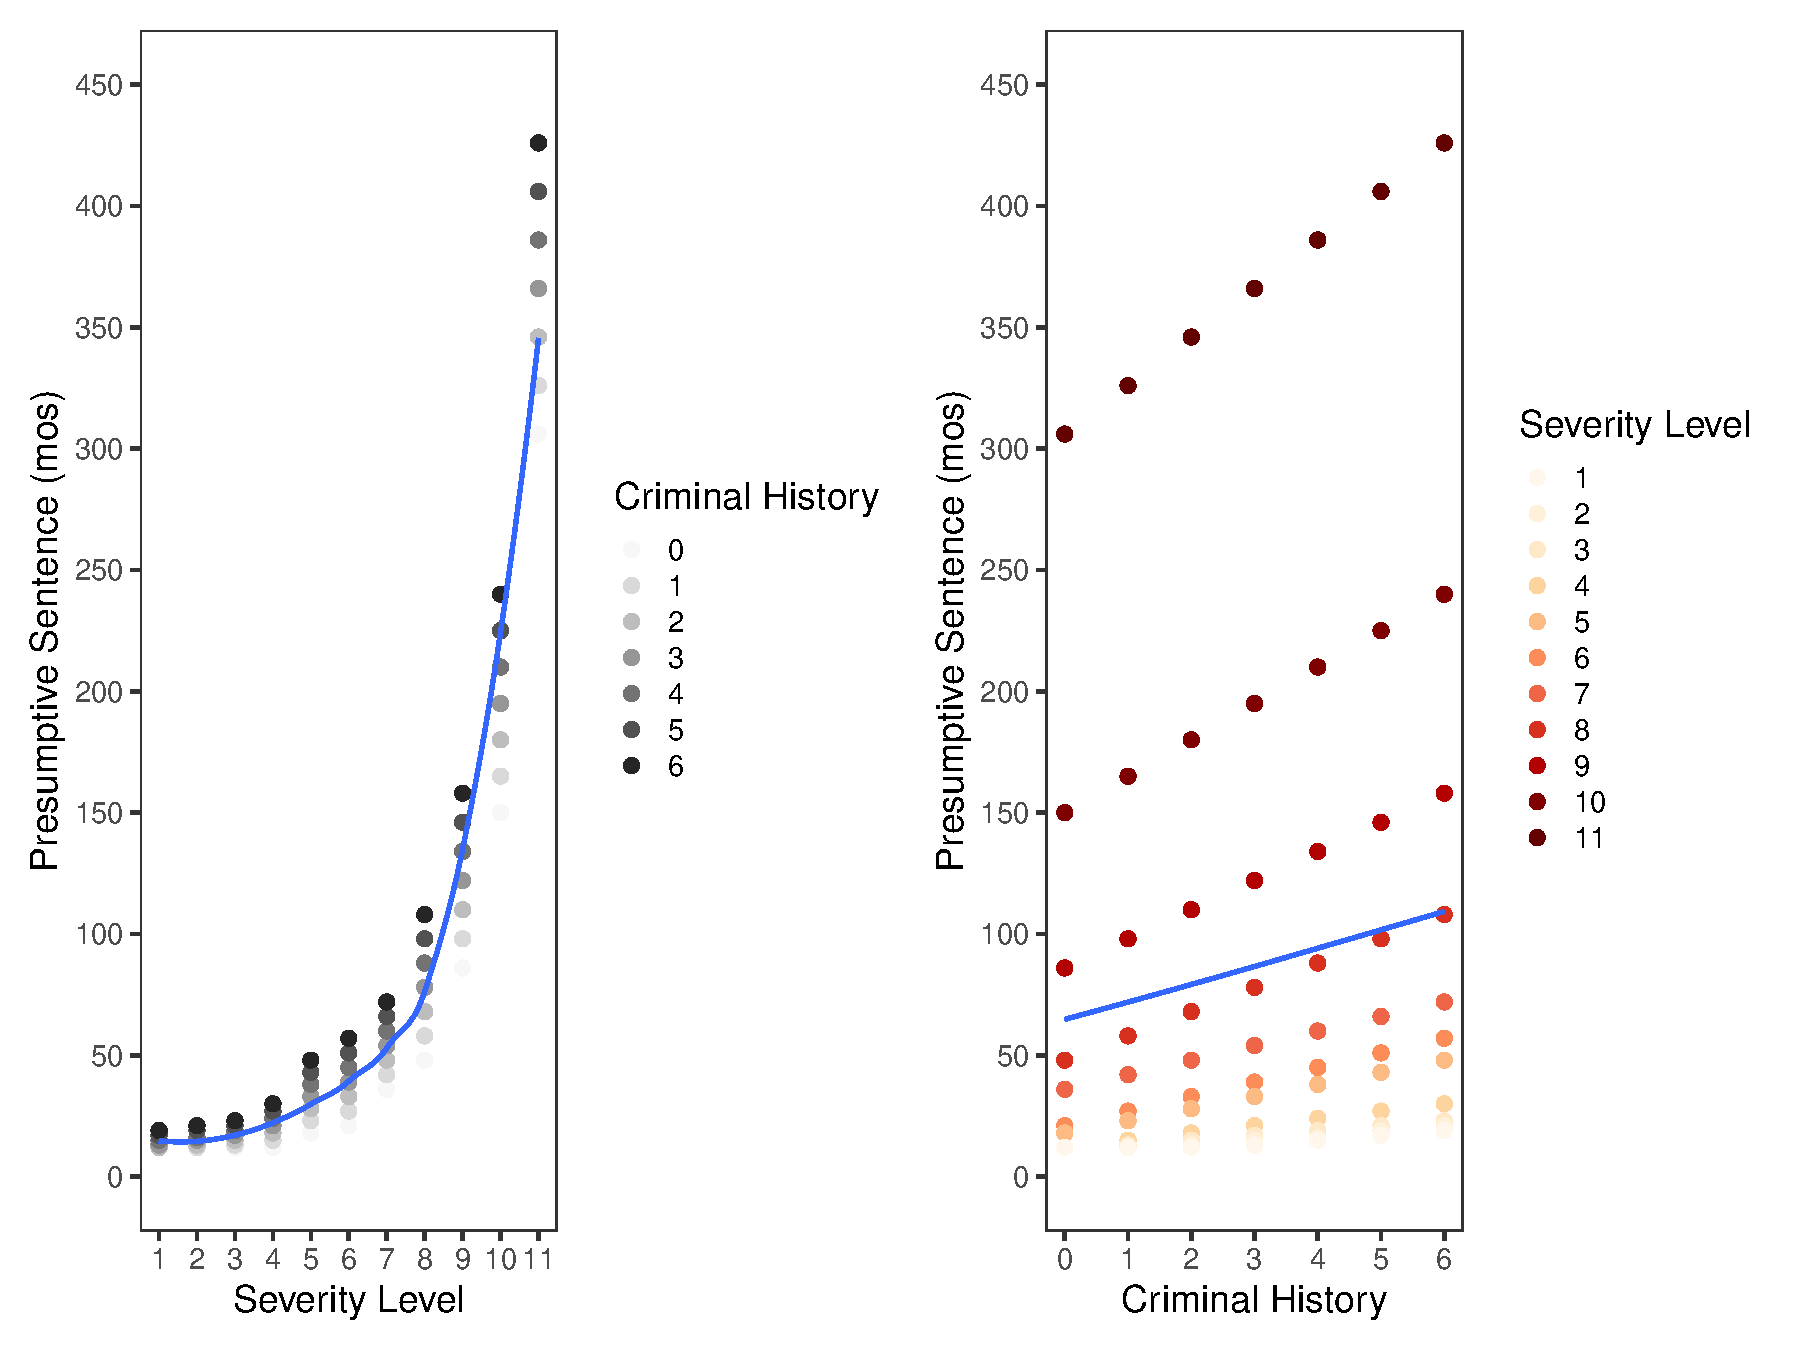
\includegraphics{sentencing_grid_files/figure-pdf/fig-scatter-1.pdf}

}

\caption{\label{fig-scatter}Scatterplot of the relationship between
felony severity level and presumptive sentence controlling for criminal
history.}

\end{figure}

\begin{verbatim}
# A tibble: 1 x 12
  r.squared adj.r.squared sigma statistic  p.value    df logLik   AIC   BIC
      <dbl>         <dbl> <dbl>     <dbl>    <dbl> <dbl>  <dbl> <dbl> <dbl>
1     0.950         0.948 0.246      697. 9.73e-49     2  0.329  7.34  16.7
# i 3 more variables: deviance <dbl>, df.residual <int>, nobs <int>
\end{verbatim}

\begin{verbatim}
# A tibble: 3 x 5
  term             estimate std.error statistic  p.value
  <chr>               <dbl>     <dbl>     <dbl>    <dbl>
1 (Intercept)         1.58    0.0733      21.6  1.18e-33
2 severity_level      0.323   0.00886     36.4  5.06e-49
3 criminal_history    0.114   0.0140       8.12 7.63e-12
\end{verbatim}

\[
\begin{split}
\mathrm{Model~1}: \hat{\mathrm{ln(Pres~Sent_i)}} &= 1.58 + 0.323(\mathrm{Off~Sev~Lev}_i) + 0.114(\mathrm{Crim~Hist}_i)
\end{split}
\]

\[
\begin{split}
\hat{\mathrm{ln(Pres~Sent_i)}} &= 1.58 + 0.323(\mathrm{Off~Sev~Lev}_i) + 0.114(\mathrm{Crim~Hist}_i)
\\[1em]
\hat{\mathrm{Pres~Sent_i}} &= e^{1.58} \times e^{0.323(\mathrm{Off~Sev~Lev}_i)} \times e^{0.114(\mathrm{Crim~Hist}_i)}
\\[1em]
\hat{\mathrm{Pres~Sent_i}} &= e^{1.58} \times e^{0.323(1)} \times e^{0.114(1)}
\\[1em]
\hat{\mathrm{Pres~Sent_i}} &= 4.85 \times 1.38 \times 1.12
\end{split}
\] The y-intercept for Model 1 is 4.85. This number cannot be
interpreted into a meaningful context, because 0 is not a felony
severity used by the Minnesota Sentencing Guidelines Commission. Each
1-unit change in \emph{offense severity level} is associated with a
\textbf{1.38-fold increase} in presumptive sentence, and each 1-unit
change in \emph{criminal history} is associated with a \textbf{1.12-fold
increase} in presumptive sentence.

\begin{figure}

{\centering 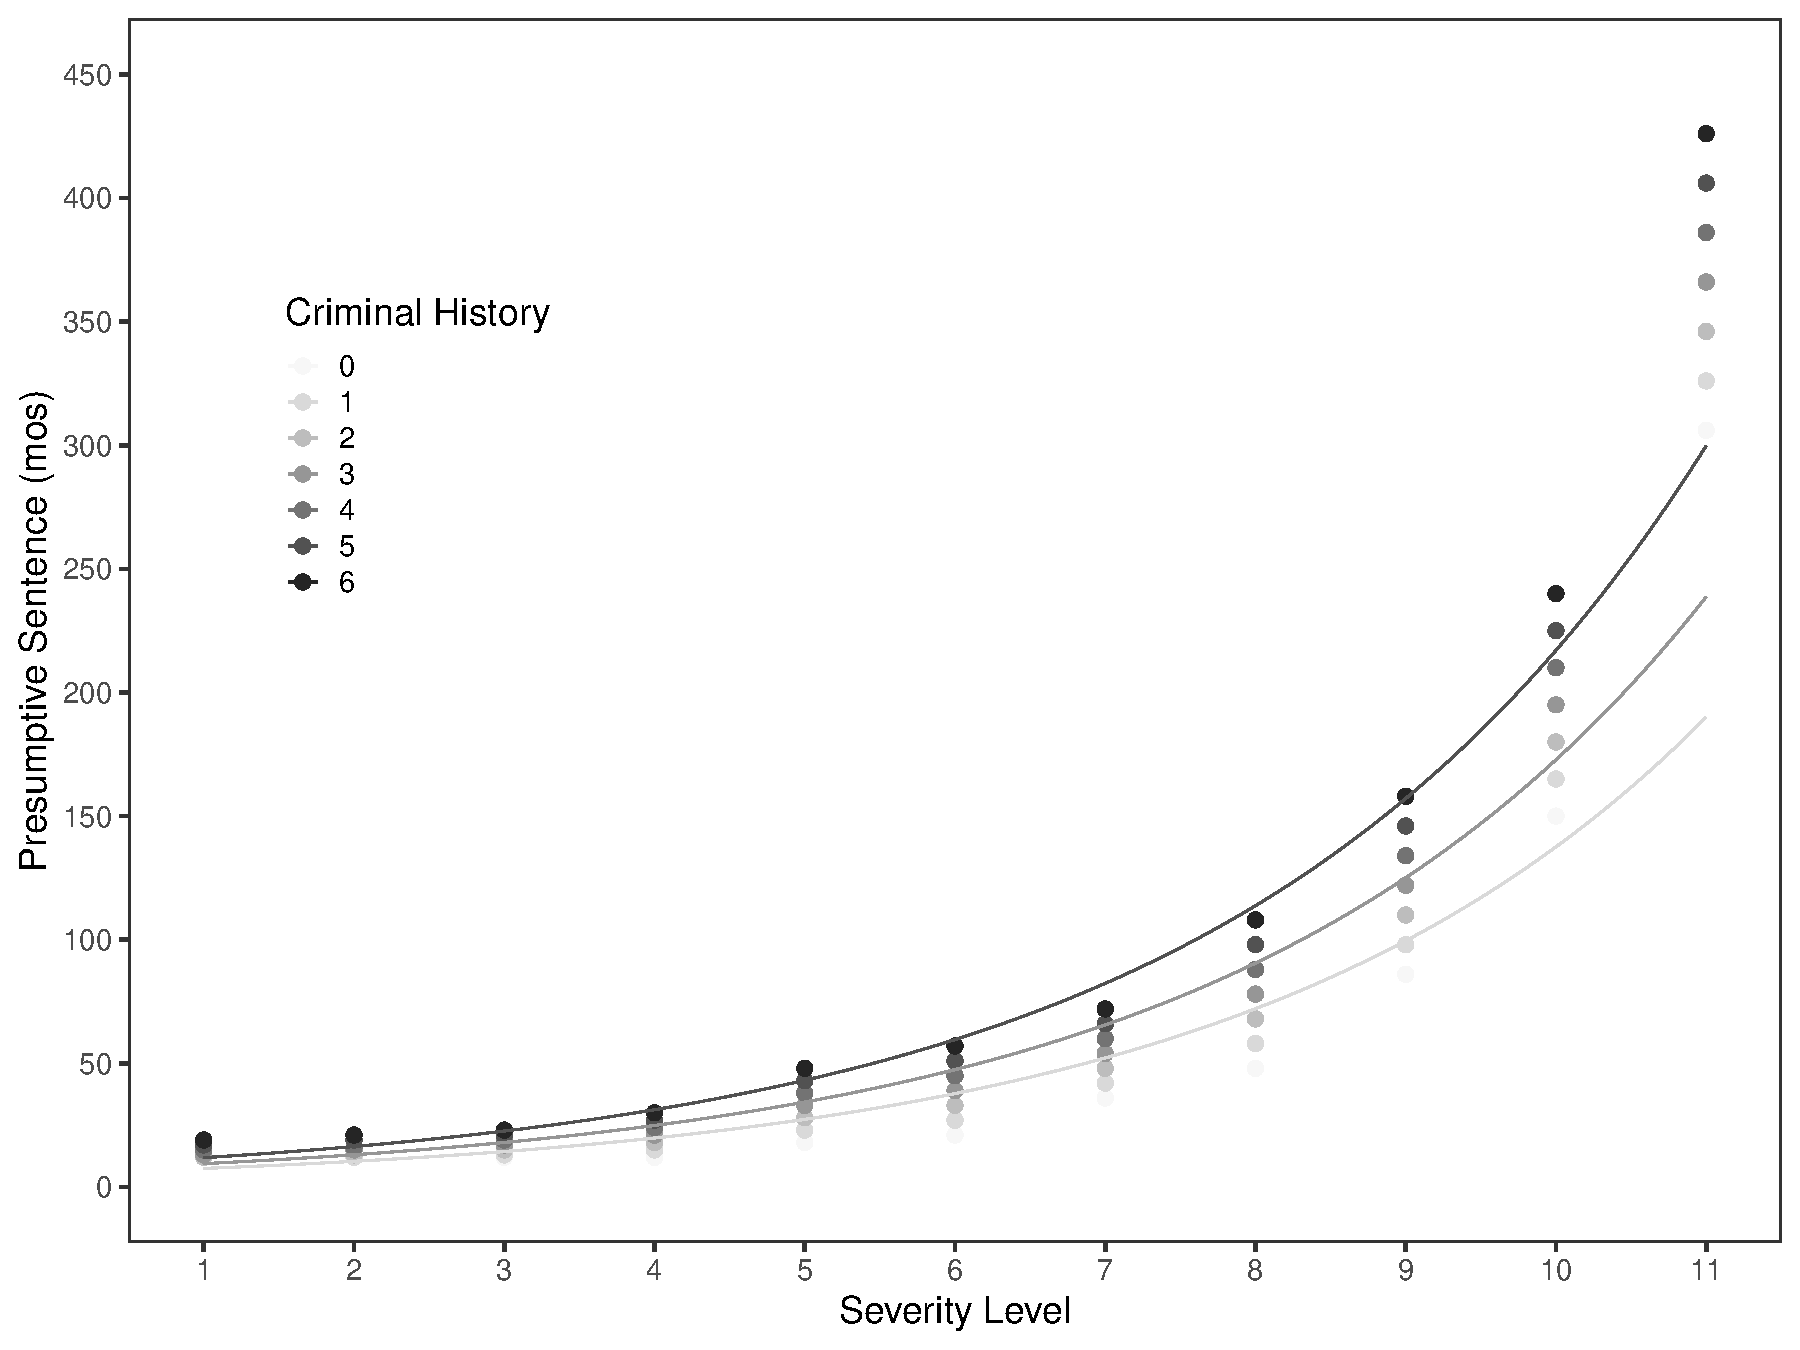
\includegraphics{sentencing_grid_files/figure-pdf/fig-fits-1.pdf}

}

\caption{\label{fig-fits}Best fits for wines from CA and wines not from
CA, according to Model 3.}

\end{figure}



\end{document}
